\documentclass[a4paper, 12pt]{report}
% Forces PDF version 1.7
\pdfminorversion=7
% Allows writing the document in english.
\usepackage[utf8]{inputenc}
\usepackage[francais]{babel}
\usepackage[T1]{fontenc}
% Allows to use images.
\usepackage{graphicx}
% Provides hyperlinks within the document.
\usepackage{enumitem}
% Adds space between paragraphs.
\usepackage{parskip}
% Supports Text Companion fonts (necessary for gensymb).
\usepackage{textcomp}
\usepackage{array}
\usepackage{multicol}
% Better tabular
\usepackage{tabularx}
% Allows to use colors.
\usepackage{xcolor}
\usepackage[margin=4cm]{geometry}
\usepackage{varwidth}
% Euro
\usepackage{eurosym}
\usepackage{amsmath}

\usepackage{subfigure}
\usepackage[
    type={CC},
    modifier={by-nc-nd},
    version={4.0},
]{doclicense}

\usepackage[colorlinks=true,urlcolor=black,linkcolor=black]{hyperref}
% New columns types
% Left
\newcolumntype{L}{>{\raggedright\arraybackslash}X}
% Center
\newcolumntype{C}{>{\centering\arraybackslash}X}
% Right
\newcolumntype{R}{>{\raggedleft\arraybackslash}X}

% Add more space before and after table
\newenvironment{centerspace}{\setlength{\topsep}{1ex}\center}{\endcenter}
% Sets the color of gray.
\newcommand{\gray}{\rowcolor[gray]{.90}}
% Allows to draw lines.
\newcommand{\HRule}{\rule{\linewidth}{0.5mm}}
% Uses the arabic numerals for sections.
\renewcommand{\thesection}{\arabic{section}}

% Width of text.
\addtolength{\textwidth}{2cm}
% Odd page left margin.
\addtolength{\oddsidemargin}{-1cm}
% Height of main text.
\addtolength{\textheight}{2cm}
% Removes indentation.
\setlength\parindent{0pt}
% Indicates overflow words.
\setlength{\overfullrule}{10pt}
% Height of items.
\setitemize{itemsep=1em}
% Adds the subsubsections in the TOC
\setcounter{tocdepth}{3}
\setcounter{secnumdepth}{3}

%%%%********************************************************************
% fancy quotes
\definecolor{quotemark}{gray}{0.7}
\makeatletter
\def\fquote{%
    \@ifnextchar[{\fquote@i}{\fquote@i[]}%]
           }%
\def\fquote@i[#1]{%
    \def\tempa{#1}%
    \@ifnextchar[{\fquote@ii}{\fquote@ii[]}%]
                 }%
\def\fquote@ii[#1]{%
    \def\tempb{#1}%
    \@ifnextchar[{\fquote@iii}{\fquote@iii[]}%]
                      }%
\def\fquote@iii[#1]{%
    \def\tempc{#1}%
    \vspace{1em}%
    \noindent%
    \begin{list}{}{%
         \setlength{\leftmargin}{0.1\textwidth}%
         \setlength{\rightmargin}{0.1\textwidth}%
                  }%
         \item[]%
         \begin{picture}(0,0)%
         \put(-15,-5){\makebox(0,0){\scalebox{3}{\textcolor{quotemark}{``}}}}%
         \end{picture}%
         \begingroup\itshape}%
 %%%%********************************************************************
 \def\endfquote{%
 \endgroup\par%
 \makebox[0pt][l]{%
 \hspace{0.8\textwidth}%
 \begin{picture}(0,0)(0,0)%
 \put(15,15){\makebox(0,0){%
 \scalebox{3}{\color{quotemark}''}}}%
 \end{picture}}%
 \ifx\tempa\empty%
 \else%
    \ifx\tempc\empty%
       \hfill\rule{100pt}{0.5pt}\\\mbox{}\hfill\tempa,\ \emph{\tempb}%
   \else%
       \hfill\rule{100pt}{0.5pt}\\\mbox{}\hfill\tempa,\ \emph{\tempb},\ \tempc%
   \fi\fi\par%
   \vspace{0.5em}%
 \end{list}%
 }%
 \makeatother

 %%%% ********************************************************************

% Starts roman numbering (trick to not numbering the first pages).
\pagenumbering{roman}

\begin{document}
\renewcommand{\bibname}{Références}
\begin{center}
  
\includegraphics[scale=0.12]{textures/logo/heh_bw.pdf}

  \vspace{1cm}

  \textsc{\LARGE Projet} \\ [0.5cm]
  \textsc{\Large Réalisation d'un site en PHP} \\ [0.5cm]

  \textsc{\large 2\up{ème} Bachelier en Informatique} \\ [0.2cm]

  \begingroup
  \fontfamily{pag} \selectfont 

  \HRule \\ [0.4cm] {
    \huge Programmation web \\ [0.2cm] 
  }
  \HRule \\ [1.3cm]
  \endgroup
  \begin{minipage}[t]{0.4 \textwidth} 
    \begin{flushleft} 
      \large \emph{Auteur:} \\ 
      Alexandre \textsc{Ducobu}
    \end{flushleft} 
  \end{minipage}
  % 
  \begin{minipage}[t]{0.4 \textwidth}
    \begin{flushright} 
      \large \emph{Enseignants :} \\ 
      Antoine \textsc{Malaise} \\
      Fabrice \textsc{Scopel}
    \end{flushright} 
  \end{minipage}

  \vspace{1cm}

  
\includegraphics[scale=0.08]{textures/logo/technical_bw.pdf}

  \vspace{0.5cm}

  Année académique 2016 - 2017
\end{center}

\thispagestyle{empty}

\newpage
\newpage
\thispagestyle{empty}
\setcounter{page}{0}
\null
\newpage
\begin{center}
  
\includegraphics[scale=0.12]{textures/logo/heh.pdf}

  \vspace{1cm}

  \textsc{\LARGE Projet} \\ [0.5cm]
  \textsc{\Large Réalisation d'un site en PHP} \\ [0.5cm]

  \textsc{\large 2\up{ème} Bachelier en Informatique} \\ [0.2cm]

  \begingroup
  \fontfamily{pag} \selectfont 

  \HRule \\ [0.4cm] {
    \huge Programmation web \\ [0.2cm] 
  }
  \HRule \\ [1.3cm]
  \endgroup
  \begin{minipage}[t]{0.4 \textwidth} 
    \begin{flushleft} 
      \large \emph{Auteur:} \\ 
      Alexandre \textsc{Ducobu}
    \end{flushleft} 
  \end{minipage}
  % 
  \begin{minipage}[t]{0.4 \textwidth}
    \begin{flushright} 
      \large \emph{Enseignants :} \\ 
      Antoine \textsc{Malaise} \\
      Fabrice \textsc{Scopel}
    \end{flushright} 
  \end{minipage}

  \vspace{1cm}

  
\includegraphics[scale=0.08]{textures/logo/technical.pdf}

  \vspace{0.5cm}

  Année académique 2016 - 2017
\end{center}

\thispagestyle{empty}

\newpage
\newpage
\thispagestyle{empty}
\setcounter{page}{0}
\null
\newpage
\newpage
\mbox{~}
\vfill
Ce document est mis à disposition selon les termes de la licence Creative
Commons “\href{https://creativecommons.org/licenses/by-nc-nd/4.0/}{Attribution
- Pas d'utilisation commerciale 4.0 International}”.

\begin{center}
  
\includegraphics[scale=1]
    {textures/images/license/license.pdf}
\end{center}
\setcounter{page}{0}
\thispagestyle{empty}

\newpage
\pagenumbering{arabic}
\tableofcontents
\newpage
\section{Présentation du projet}
\label{sec:presentation}


\subsection{Introduction}
\label{sec:intro}

Dans le cadre du cours de \textbf{Programmation web}, il nous a été demandé de réaliser un site dynamique en PHP.\\
Dans le cadre d'un site dynamique, les données disponibles sur le site proviennent d'une base de données, ici, composée de trois tables.


\subsection{Énoncé}
\label{sec:enonce}

Le site doit comprendre une base de données composée de trois tables.\\

L'une d'elles est prévue pour la gestion des utilisateurs, représentés par, au minimum, un nom, un prénom, une adresse mail et un mot de passe.\\
L'adresse mail doit servir pour la connexion au site, et le mot de passe a une longueur minimale de 4 caractères.\\

Du côté des fonctionnalités, les utilisateurs doivent pouvoir se (dé)connecter, modifier leurs données, supprimer leur compte et contacter l'administrateur.\\
L'\textbf{administrateur}, utilisateur créé par nos soins, a accès à toutes les données de la base de données, peut ajouter et modifier du contenu, réinitialiser le mot de passe des utilisateurs et peut aussi les bannir.


\subsection{Description}
\label{sec:description}

Ce site proposera aux visiteurs de s'inscrire afin de créer une liste privée de médicaments et ce, d’après une liste de médicaments \textit{non-exhaustive}.\\
Cette liste sera établie par l'administrateur selon son envie et les demandes envoyées par les utilisateurs.\\

Chaque médicament comprendra: sa posologie, les effets néfastes, les contre-\\indications ainsi qu'un lien vers sa notice.\\

Les personnes n’ayant pas de compte auront accès à la liste des médicaments ne contenant que leur nom et leur posologie.

\newpage


\subsection{Langages}
\label{sec:langages}

Les deux langages principaux sont donc, vu l'énoncé, le \textbf{PHP} et \textbf{MySQL}.\\
Ceux-ci sont, bien entendu, accompagnés du HTML, CSS ainsi que du JavaScript \textit{(et jQuery)} pour la création du site.

\vspace{1cm}

\begin{figure}[!h]
\centering
\begin{minipage}[c]{0.4\textwidth}
  \centering
  
\includegraphics[scale=0.15]
  {textures/images/tools/php.pdf}
\caption{Logo de PHP}\label{php}
\end{minipage} \qquad
\begin{minipage}[c]{0.4\textwidth}
  \centering
  
\includegraphics[scale=0.15]
  {textures/images/tools/mysql.pdf}
\caption{Logo de MySQL}\label{mysql}
\end{minipage}
\end{figure}


\subsection{Outils}
\label{sec:outils}

D'après le cours de bases de données du premier quadrimestre et le système d'exploitation utilisé, l'outil choisi pour le serveur web ainsi que la base de données est \textbf{MAMP}.\\
En ce qui concerne l'éditeur de texte, c'est \textbf{Atom} qui a été retenu pour sa simplicité ainsi que pour la familiarité que je ressent envers lui.

\vspace{1cm}

\begin{figure}[!h]
\centering
\begin{minipage}[c]{0.4\textwidth}
  \centering
  
\includegraphics[scale=0.15]
  {textures/images/tools/mamp.pdf}
\caption{Logo de MAMP}\label{mamp}
\end{minipage} \qquad
\begin{minipage}[c]{0.4\textwidth}
  \centering
  
\includegraphics[scale=0.15]
  {textures/images/tools/atom.pdf}
\caption{Logo de Atom}\label{atom}
\end{minipage}
\end{figure}


%%% Local Variables:
%%% mode: latex
%%% TeX-master: t
%%% End:

\newpage
\section{Base de données}
\label{sec:BD}


\subsection{Création de la base de données}
\label{sec:creation-db}

La base de données est composée de trois tables contenant toutes les données utiles au bon fonctionnement du site.\\
Il y a la table \textbf{Users} \textit{pour tout ce qui concerne les utilisateurs}, la table \textbf{Medicines}, \textit{qui concerne les médicaments} et le table \textbf{Reserves} \textit{qui contient la réserve de chaque utilisateur}.

\begin{figure}[h]
  \centering
  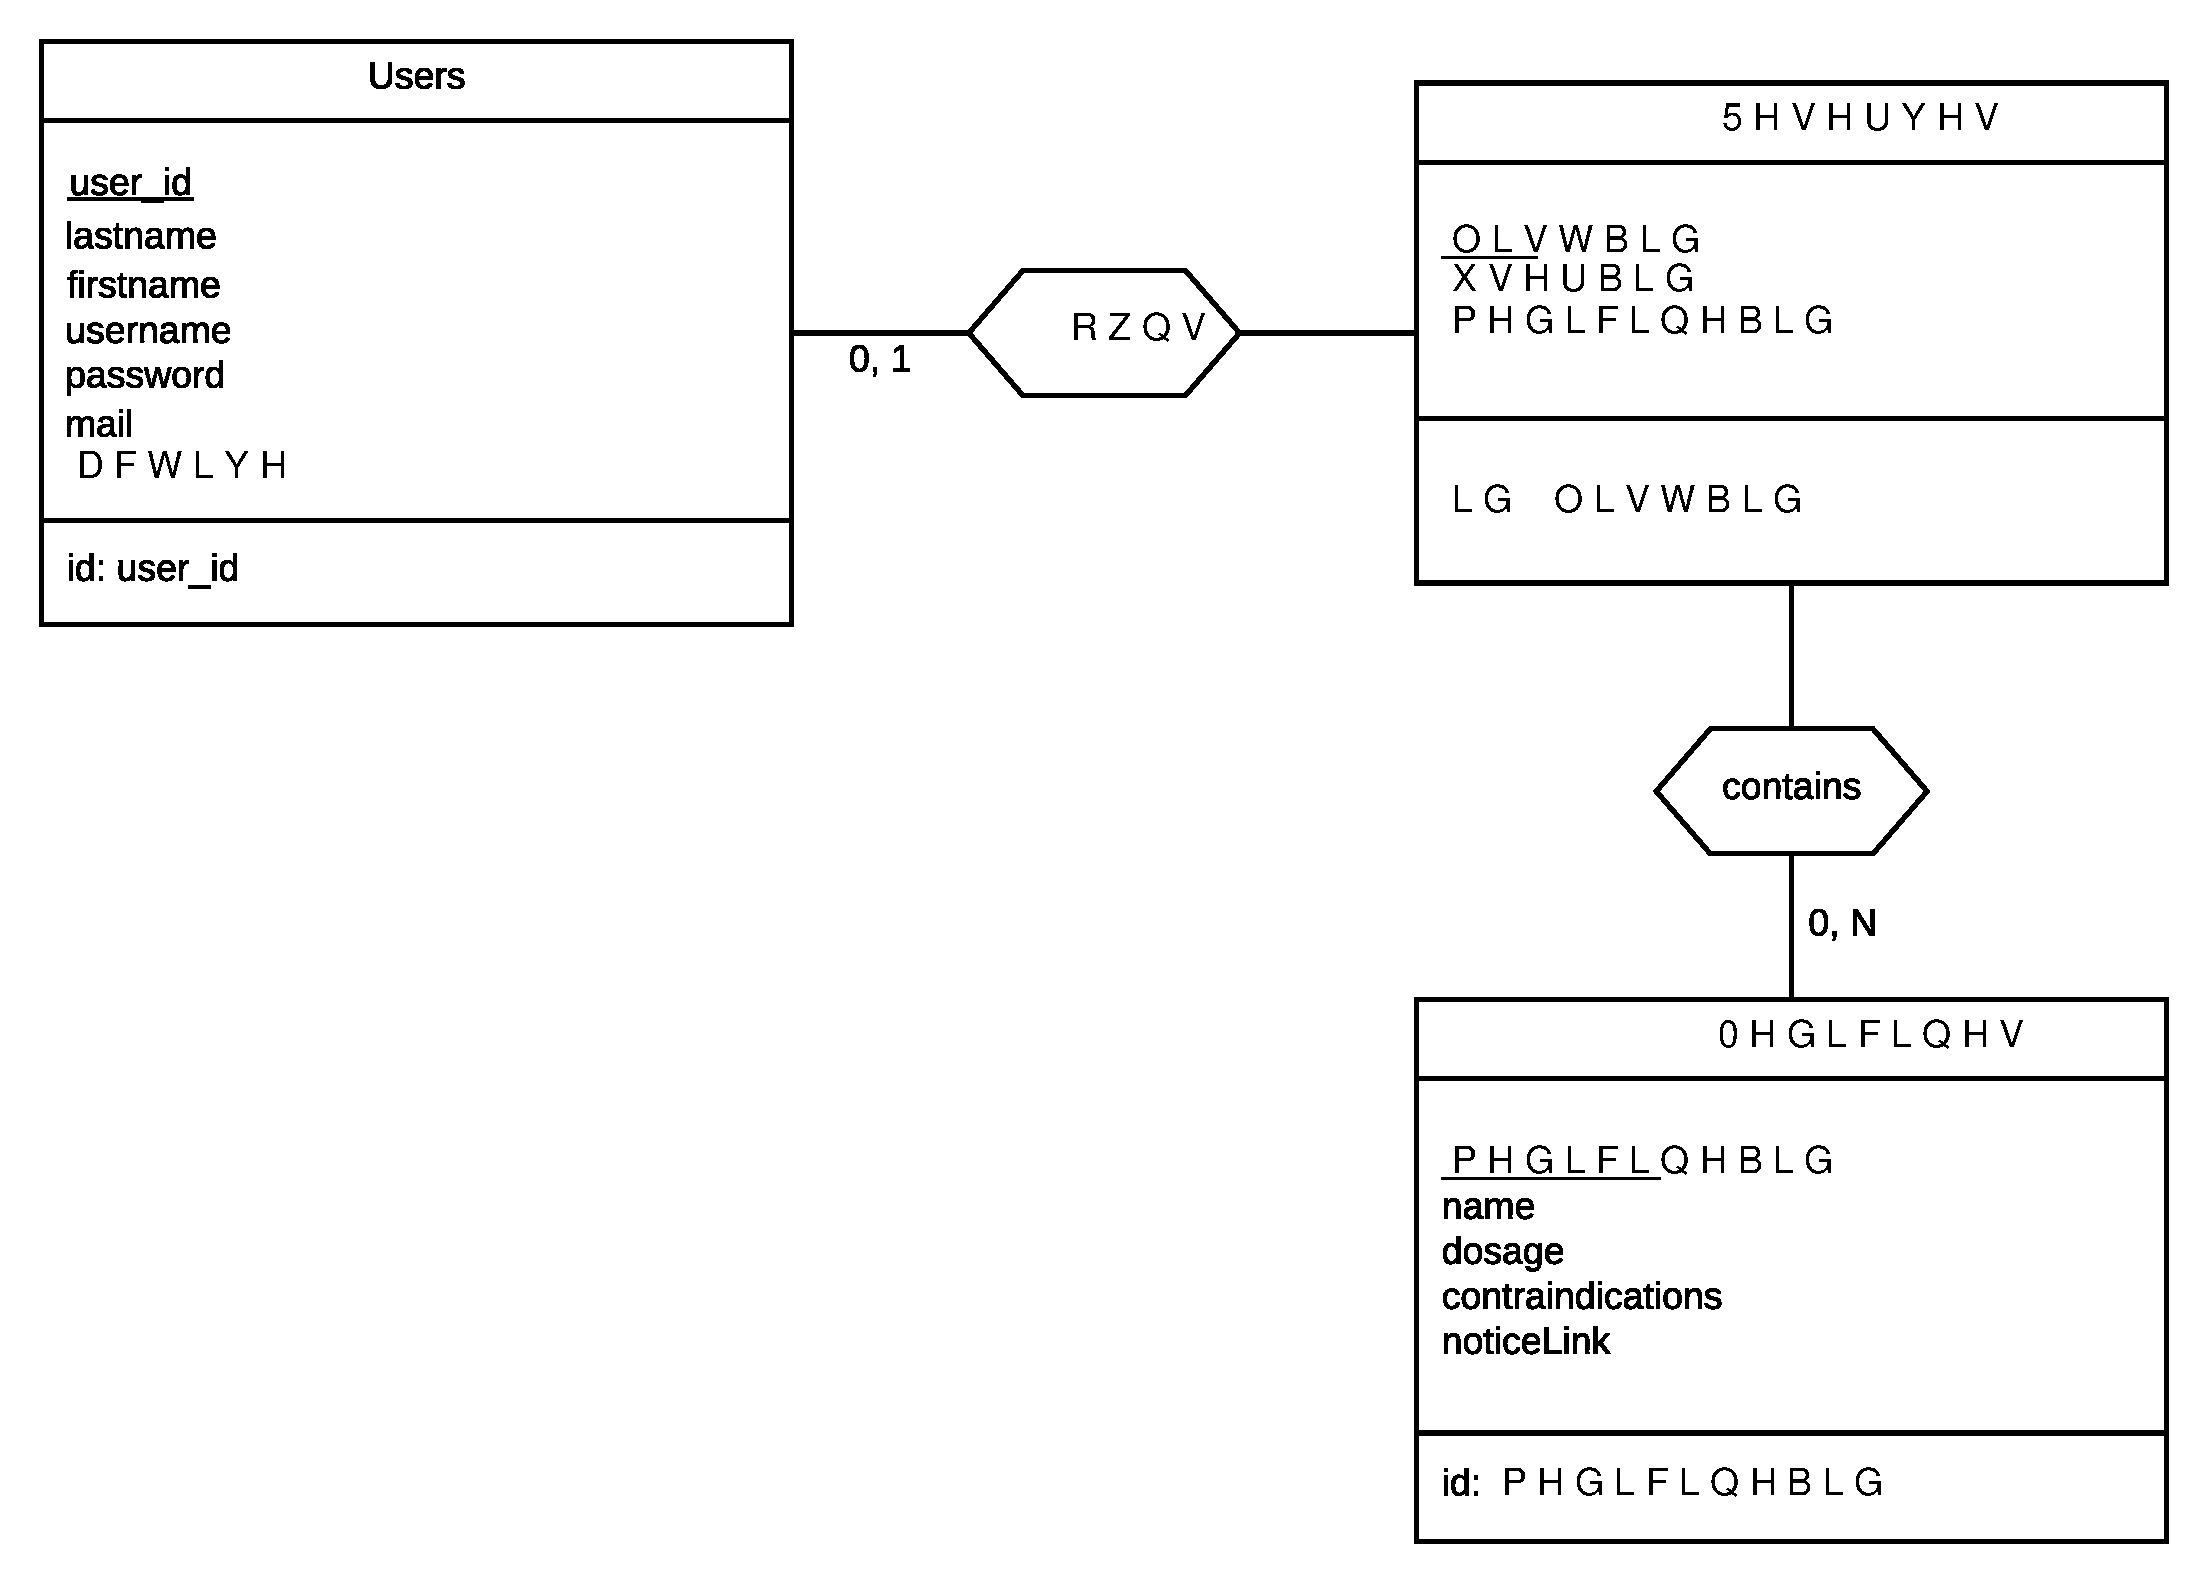
\includegraphics[scale=0.4]
  {textures/images/db/DB.pdf}
  \caption{Schéma conceptuel de la base de données}
  \label{fig:db}
\end{figure}

\newpage

\subsection{Vue détaillée}
\label{sec:vue-details}


\subsubsection{Table Medicines}
\label{sec:table-med}

Cette table contient les informations de chaque médicament.\\

\begin{itemize}
    
    \item[$\bullet$] \textbf{medicine\_id} est l'identifiant du médicament.\\
    Il sert de clé primaire de la table et est auto-incrémenté à partir de 1.
    
    \item[$\bullet$] \textbf{name} est le nom du médicament.\\
    Ce champ, en plus de contenir le médicament, identifie son type: comprimé, comprimé effervescent, gélule, etc.
    
    \item[$\bullet$] \textbf{dosage} contient le ou les différents dosages possibles \textit{(en mg ou en g)}.
    
    \item[$\bullet$] \textbf{contraindications} comprend deux à trois lignes de contre-indications du médicament.
    
    \item[$\bullet$] \textbf{noticeLink} contient l'adresse vers la notice en ligne, à télécharger.
    
\end{itemize}

\textbf{\textit{Remarque : }} l'image représentant le médicament est sauvegardée dans un dossier spécifique et est liée à son identifiant.\\
Elle ne se trouve donc pas dans la base de données.


\subsubsection{Table Reserves}
\label{sec:table-res}

Cette table lie les deux autres: la réserve de médicaments lie chaque utilisateur à ses médicaments.\\

\begin{itemize}

    \item[$\bullet$] \textbf{list\_id} est l'identifiant unique de la réserve.\\
    Il est auto-incrémenté à partir de un et sert de clé primaire.
    
    \item[$\bullet$] \textbf{user\_id} est l'identifiant de l'utilisateur.\\
    C'est une clé étrangère.
    
    \item[$\bullet$] \textbf{medicine\_id} identifie les médicaments.\\
    C'est aussi une clé étrangère.
    
\end{itemize}

\newpage

\subsubsection{Table Users}
\label{sec:table-users}

C'est la table contenant les données de chaque utilisateur ainsi que l'état de leur compte.\\

\begin{itemize}
    
    \item[$\bullet$] \textbf{user\_id} est l'identifiant unique du médicament.\\
    Il sert de clé primaire de la table et est auto-incrémenté à partir de un.
    
    \item[$\bullet$] \textbf{lastname} est le nom de famille de l'utilisateur.
    
    \item[$\bullet$] \textbf{firstname} est le prénom de l'utilisateur.
    
    \item[$\bullet$] \textbf{username} est le nom d'utilisateur unique choisi lors de l'inscription.
    
    \item[$\bullet$] \textbf{password} est le mot de passe de l'utilisateur.\\
    Il a une taille minimale de 4 caractères et est haché \footnote{\url{https://fr.wikipedia.org/wiki/Fonction\_de\_hachage\_cryptographique}} \textit{(et salé)} à l'aide de SHA512.
    
    \item[$\bullet$] \textbf{mail} contient l'adresse mail de l'utilisateur.\\
    Ce champ est unique, vu qu'il sert à la connexion de l'utilisateur.
    
    \item[$\bullet$] \textbf{active} donne l'état du compte de l'utilisateur:
    
    \begin{itemize}
        
        \item \textbf{0} indique que le compte est inactif.\\
        Cela signifie que le compte a été supprimé ou que l'administrateur a banni l'utilisateur.
        
        \item \textbf{1} indique que le compte est actif \textit{(par défaut)}.
        
    \end{itemize}
    
\end{itemize}


%%% Local Variables:
%%% mode: latex
%%% TeX-master: t
%%% End:
\newpage
\section{Site}
\label{sec:site}


\subsection{Arborescence}
\label{sec:arborescence}

Le site a été divisé en neuf dossiers pour plus de clarté.

\begin{itemize}

    \item[$\bullet$] Trois d’entre-eux ne sont pas liés au PHP:
    \begin{itemize}
    
         \item \textbf{img :} contient toutes les images du site.
         
         \item \textbf{js :} contient les différents scripts en JavaScript ainsi que jQuery.
         
         \item \textbf{style :} contient les différents fichiers contenant le CSS du site.
         
    \end{itemize}
    
    \item[$\bullet$] Ensuite, viennent les six autres qui contiennent le PHP:
    \begin{itemize}
    
         \item \textbf{actions :} contient les scripts php liés aux actions telles que la\\ (dés)activation d’un compte, l’ajout d’un médicament ainsi que la ré-initialisation d’un mot de passe.
         
         \item \textbf{connexion :} contient les scripts php liés à la connexion à la base de données ainsi que la (dé)connexion au site.
         
         \item \textbf{DB :} contient les scripts MySQL qui créent et initialisent la base de données.
         
         \item \textbf{forms :} contient les différents formulaires (avec leur version de vérification) tels que celui de l’ajout/modification d’un médicament, de\\ connexion, etc.
         
         \item \textbf{include :} contient les scripts php formant une partie des pages comme le pied de page et les différentes tables de la base de données.
         
         \item \textbf{insidePages :} les pages internes du site comme la page principale, celle de changement de mot de passe, etc.
         
    \end{itemize}
    
    \item[$\bullet$] Pour finir, l’index et la page d’erreur de connexion à la base de données se trouvent à la racine du site.

\end{itemize}

\newpage


\subsection{Arborescence détaillée}
\label{sec:arb-details}

Voici maintenant chaque dossier détaillé.


\subsubsection{Dossiers non liés au PHP}
\label{sec:folder-no-php}

Le dossier \textit{js} contient trois fichiers.\\

Le premier, \textbf{\textit{jquery-3.1.1.min.js}}, contient toutes les fonctions de jQuery.\\

Le second, \textbf{\textit{jquery.cslide.js}}, est une librairie permettant d’insérer facilement un slider \footnote{\url{http://callmenick.com/post/responsive-content-slider}}.\\
Il est utilisé pour afficher le contenu des tables 5 par 5 grâce à l’utilisation de boutons \guillemotleft \ Suivant \guillemotright \ et \guillemotleft \ Précédent \guillemotright.\\

Le troisième et dernier, \textbf{\textit{script.js}},contient trois fonctions:
\begin{enumerate}

    \item hideUsers(): qui cache l'onglet \textit{Utilisateurs} lorsqu'un utilisateur autre que l'administrateur est connecté.
    
    \item setCurrentTab(): qui sélectionne l'onglet courant.
    
    \item updateFooterBg(): qui change la couleur de fond du footer sur les autres navigateurs que Safari, qui permet d'avoir un fond flouté.
    
\end{enumerate}


\subsubsection{Dossiers PHP}
\label{sec:folder-php}

Le dossier \textbf{actions} est constitué de quatre fichiers PHP.

\begin{itemize}

    \item \textbf{\textit{activateUser.php}}, qui permet de désactiver le compte d’un utilisateur ou de le réactiver.\\
    Tous les utilisateurs, à l’exception de l’administrateur, peuvent désactiver leur compte.\\
    L’administrateur, lui, a le droit d’activer ou de bannir \textit{(désactiver)} le compte de n’importe quel utilisateur sauf le sien.
    
    \item \textbf{\textit{addMedToList.php}}: ce fichier reçoit donc les données d’un nouveau médicament qu’il ajoute à la base de données.
    
    \item \textbf{\textit{changeDBData.php}}: il a un fonctionnement proche du précédent, sauf qu’il modifie les données de l’utilisateur (nom de famille, prénom et adresse mail).
    
    \item \textbf{\textit{reinitPWD.php}}: appelé par l’administrateur, ce fichier réinitialise le mot de passe de l’utilisateur sélectionné en lui donnant une valeur par défaut \textit{(EpcCM98)}.

\end{itemize}

\newpage

Le dossier \textbf{connexion} en possède douze.

\begin{itemize}

    \item \textbf{\textit{connexion.php}} contient le script de connexion à la base de données.
    
    \item \textbf{\textit{dbInfos.php}} contient les données de connexion à la base de données: nom d’hôte, nom de la base, nom d’utilisateur, mot de passe et numéro de port.
    
    \item \textbf{\textit{login.php}} est le script appelé pour vérifier le login lors d’une tentative de connexion au site.
    
    \item \textbf{\textit{loginPage.php}}: c’est la page de connexion au site. C’est elle qui appelle le script précédent.
    
    \item \textbf{\textit{logout.php}}: comme son nom l’indique, il est utilisé pour déconnecter l’utilisateur du site.
    
    \item \textbf{\textit{signUp.php}}: son fonctionnement proche de celui de login.php lui permet d’enregistrer un nouvel utilisateur.
    
    \item \textbf{\textit{signuPage.php}}: c’est la page d’inscription au site. C’est elle qui appelle le script précédent.
    
    \item Les cinq suivant servent à vérifier les données des formulaires à l’aide de regex\footnote{\href{https://fr.wikipedia.org/wiki/Expression\_rationnelle}{Expression régulière (en anglais: \textbf{Reg}ular \textbf{ex}pression)}}.\\
    Il est aussi parfois nécessaire de vérifier des données dans la base de données comme le nom d’un médicament lors de son ajout afin de ne pas avoir de doublons.\\

\end{itemize}

Le dossier \textbf{BD} est le plus simple, car il ne contient que deux fichiers SQL:

\begin{itemize}

    \item \textbf{\textit{CreateDB.sql}} crée la base de données ainsi que les trois tables la composant.
    
    \item \textbf{\textit{InitDB.sql}} initialise la base de données en ajoutant trois utilisateurs dont l’administrateur; ajoute sept médicaments différents; et remplit la réserve des deux utilisateurs créés.

\end{itemize}

\newpage

Le dossier \textbf{forms} contient tous les formulaires du site.\\

En résumé, chaque formulaire existe en deux formes:
\begin{itemize}
    
    \item[$\bullet$] Le formulaire vierge qui, une fois soumis, est vérifié par l’un des scripts de vérification du dossier connexion.
    
    \item[$\bullet$] Le formulaire de vérification qui, si les données sont acceptées, appelle le script adéquat.\\
    Dans le cas contraire, le formulaire est affiché avec les bonnes données et/ou les messages d’erreurs pour chaque champ.\\
    
\end{itemize}

Le dossier \textbf{include} contient 8 fichiers.

\begin{itemize}
    
    \item \textbf{\textit{footer.php}} contient le footer avec ou sans le moyen de contacter l’administrateur selon que l’on soit connecté ou non et que l’on soit l’administrateur ou non.
    
    \item Les deux fichiers de barre de navigation:
    \begin{itemize}
        
        \item \textbf{\textit{navBarConnect.php}} permet d’afficher la liste des médicaments et les liens de connexion et d’inscription au site.
        
        \item \textbf{\textit{navBarReserve.php}}: affichée lorsque l’utilisateur est connecté, elle permet de naviguer entre les différentes tables de la base.
        
    \end{itemize}
    
    \item \textbf{\textit{medsPopUp.php}} permet d’afficher les données des médicaments dans un popup.
    
    \item \textbf{\textit{account.php}} affiche les données de l’utilisateur et lui permet de les changer ou de supprimer son compte.
    
    \item Les trois derniers permettent d’afficher les données contenues dans les différentes tables d’après l’utilisateur connecté.
    
\end{itemize}

\newpage

Le dernier dossier est intitulé \textbf{insidePages}, car il est constitué des différentes pages disponibles lorsque l'utilisateur est connecté.

\begin{itemize}
    
    \item \textbf{\textit{chgMed.php}} est la page qui permet d’ajouter ou de modifier un médicament à la base.
    
    \item \textbf{\textit{chgPwd.php}} permet de changer de mot de passe.
    
    \item \textbf{\textit{chooseImage.php}} propose de choisir une image \textit{(png)} pour son médicament.
    
    \item \textbf{\textit{page.php}} est la page la plus utilisée du site: c’est elle qui permet de consulter les données de la base, de changer ses données personnelles et de supprimer son compte.
    
    \item \textbf{\textit{productList.php}} est la page qui permet de consulter la liste des médicaments sans être connecté.
    
\end{itemize}


\subsubsection{Dossier racine}
\label{sec:folder-root}

Le fichier \textbf{\textit{index.php}} affiche, comme on peut s’en douter, la page d’accueil du site qui permet de se connecter et de s’inscrire au site, et d’afficher la liste des médicaments.\\

La page d’erreur de connexion à la base de données, \textbf{\textit{DBerror.php}}, affiche un message d’erreur \textit{(erreur 503)} lorsqu’il y a une erreur de connexion à la base de données.

\newpage


\subsection{Connexion à la base de données}
\label{sec:conn-bd}

En ce qui concerne la connexion à la base de données, aucun \textit{design pattern} n’a été utilisé, car, lorsque cette matière a été abordée au cours, la majeure partie du projet était déjà achevée.\\

Le type de requêtes utilisé pour l'accès à la base de données est le type PDO.\\
De manière plus précise, ce sont des requêtes préparées qui ont été utilisées pour plus de sécurité \textit{(voir la section~\ref{sec:securite}\textbf{~\nameref{sec:securite}})}.\\
De plus, PDO permet plus de flexibilité, est recommandée, très utilisée \textit{(et possède donc une importante communauté)} et est enseignée à l'école.\\

On pourrait alors ajouter, dans les évolutions possibles, le passage à la \textit{programmation orientée objet}, couplée à l’utilisation du \textit{singleton} et, comme structure de site, l’utilisation du \textit{design pattern \textbf{MVC}}.

\newpage


\subsection{Sécurité}
\label{sec:securite}

Pour la sécurité du site tout accès à la base de données passe par des requêtes préparées \textit{(PDO)}, car celles-ci protègent le site de toute injection SQL.\\

La connexion au site est surveillée grâce à la mise en place d’une session. Dès qu’un accès à une page se fait, la connexion est vérifiée. Si l’utilisateur n’est pas identifié, il est redirigé vers la page d’accueil.\\

En plus de cela, chaque champ de formulaire est protégé par des expressions régulières \textit{(regex)}.\\
Celles-ci vérifient que les données entrées sont de la forme voulue: un nom ne doit contenir que des lettres et, selon une certaine forme, peut être divisé à l’aide d’un trait d’union; une adresse mail ne contient que des lettres minuscules non-accentuées, des points et un seul arobase; etc.\\

De plus, les mots de passe ont une longueur minimale de quatre caractères et doivent contenir, au moins, une majuscule, un minuscule et un chiffre.\\
Ils sont aussi hachés à l’aide de \textit{SHA512} et d’un \textit{salage dynamique} pour plus de sécurité.\\
En effet, le mot de passe est de la forme \textbf{+\%\# longueur mot\_de\_passe  ¨*§}.\\ Par exemple, le mot de passe \textbf{Test1} devient \textbf{+\%\#5Test1¨*§} avant d’être haché.\\
Il est ainsi indéchiffrable, mais cela a aussi pour effet de sécuriser la base de données puisque le résultat ne contiendra que des caractères sûrs.

%%% Local Variables:
%%% mode: latex
%%% TeX-master: t
%%% End:

\newpage
\section{Conclusion}
\label{sec:conclusion}


\subsection{Résultat}
\label{sec:resultat}

Le site propose donc à chacun de créer un compte afin de posséder sa liste de médicaments.\\

Un utilisateur, identifié par son adresse mail et son nom d'utilisateur, peut modifier ses données depuis la page \textit{Compte}.\\
Il peut ainsi modifier son nom de famille, son prénom, son adresse mail et son mot de passe. Il a aussi la possibilité de supprimer son compte.\\

L'administrateur peut être contacté par les utilisateurs du site que ce soit pour ajouter un médicament ou pour réinitialiser leur mot de passe.\\ Il peut aussi bannir des utilisateurs.\\
En plus d'ajouter des médicaments, il a bien sûr la possibilité de les modifier, mais pas de les supprimer.
En effet, un utilisateur possédant un médicament sur le point d'être supprimé serait mécontent de le perdre.\\
Comme les autres utilisateurs, il peut changer ses données, mais il ne peut pas supprimer son compte, étant donné qu'il est l'administrateur.\\

Les visiteurs du site ne possédant pas de compte ont la possibilité de parcourir la liste des différents médicaments disponibles.\\

Il est à remarquer que, d'après les bonnes pratiques des bases de données, il ne faut pas supprimer les données mais les rendre invisibles aux utilisateurs.\\
Cette pratique est utilisée lors de la suppression d'un compte qui n'est pas supprimé, mais simplement désactivé.


\subsection{Différences avec le cahier des charges}
\label{sec:diff-cahier}

Lors de la création de la maquette du site, l'utilisation d'avatars pour identifier les utilisateurs s'est avérée moins intéressante et utile qu'escompté.\\
En effet, les utilisateurs n'ayant pas d'interactions entre-eux et ne communiquant avec l'administrateur que par mails, les avatars sont devenus superflus.\\

Lors de la conception de la version préliminaire, il est apparu que les effets néfastes et les contre-indications étaient souvent similaires.\\
J'ai alors pris la décision de les regrouper afin d'éviter les doublons.

%%% Local Variables:
%%% mode: latex
%%% TeX-master: t
%%% End:
\newpage
\newpage
\thispagestyle{empty}
\setcounter{page}{0}
\null
\newpage
\end{document}
